% !TeX root = ../main.tex

\section{Homework \#5}

\begin{problem}
  根据 Landau 理论,超导体 Gibbs 自由能密度在超导 -- 正常金属态临界点可展开为
  \[
    g_s(n_s) = g_n + \alpha n_s + \frac\beta2 n_s^2 + \cdots.
  \]
  其中 $n_s$ 是超导电子密度, $g_n$ 是正常金属的 Gibbs 自由能密度.
  当 $T \geq T_c$, $n_s = 0$. 由于超导态有序态, $g_s(n_s) \leq g_n$.
  当 $T < T_c$, $\alpha(T) < 0$, 且 $\alpha(T_c) = 0$.
  \begin{enumext}
    \item 写出 $\alpha(T)$ 在 $T \sim T_c$ 附近的一般形式.
    \item 说明在 $T \sim T_c$ 附近可取 $\beta(T) \approx \beta(T_c)$.
    \item 由 $\odv{g_s}{n_s} = 0$ 求出 Gibbs 自由能极值.
    \item 利用 (c) 的结果和 $g_n - g_s = \mu_0H_c^2(T)/2$ ($H_c$ 是超导临界磁场)
    求 $H_c(T)$ 与 $(T_c - T)$ 的关系.
  \end{enumext}
\end{problem}
\begin{solution}\leavevmode
  \begin{enumext}
    \item In the continuous phase transition, $\alpha(T_c) = 0$ and linear
    to $T$ around $T_c$. Then, its universe form is
    \[
      \alpha(T) = \alpha_0(T - T_c) + O((T - T_c)^2).
    \]
    \item Comparaing to $\alpha(T)$, the change of $\beta(T)$ is high-order.
    Then, under the 1st order approximation, one can
    take $\beta(T) \approx \beta(T_c)$.
    \item Keep the second order of $g_s$. Then
    \[
      0 = \alpha + \beta n_{s0}, \quad n_{s0} = -\frac\alpha\beta.
    \]
    Substituting it into $g_s$, then the peak value of the Gibbs free energy is
    \[
      g_s = g_n + \alpha n_{s0} + \frac\beta2 n_{s0}^2
          = g_n - \frac{\alpha^2}{2\beta}.
    \]
    \item From (c), one can obtain
    \[
      g_n - g_s = \frac{\alpha^2}{2\beta} = \frac{\mu_0H_c^2(T)}{2}, \quad
      H_c^2(T) = \frac{\alpha^2}{\mu_0\beta}
      \xlongequal{\alpha(T) \approx \alpha_0(T - T_c)}
      \frac{\alpha_0}{\sqrt{\mu_0\beta}} (T_c - T).
    \]
  \end{enumext}
\end{solution}

\begin{problem}
  比较超导相变与顺磁--铁磁相变, 讨论超导相变. (什么情况下是一级相变? 什么情况下是二级相变?)
\end{problem}
\begin{solution}\leavevmode
  \begin{enumext}
    \item 超导相变
    \begin{enumext}
      \item 二级相变: 常规情况 (如 BCS 超导体), 序参量连续增长.
      \item 一级相变: 当相变伴随晶体晶格对称性改变 (即 B1g 对称性破缺) 时,
      例如某些非常规超导体.
    \end{enumext}
    \item 顺磁-铁磁相变
    \begin{enumext}
      \item 二级相变: 常见于各向同性 (如海森堡模型) 或短程相互作用的系统, 在平均场理论下.
      \item 一级相变: 通常由淬火无序, 竞争序或长程相互作用导致.
    \end{enumext}
  \end{enumext}
\end{solution}

\begin{problem}[林宗涵《热力学与统计物理》 9.1]
  范德瓦尔斯方程的另一种推导方法是作平均场近似. 设气体的哈密顿量为
  \[
    H = \sum_{i=1}^N \frac{\bm p_i^2}{2m} + \sum_{i<j} \phi(r_{ij}),
  \]
  今假设第 $i$ 个分子所受其他分子的相互作用可以用平均场 $\phi_\text{mf}(\bm r)$
  来近似表达, 即 $H$ 近似用下列平均场哈密顿量代替
  \[
    H_\text{mf} = \sum_{i=1}^N \ab\{\frac{\bm p_i^2}{2m}
                + \phi_\text{mf}(\bm r_i)\}.
  \]
  现作为对平均场的进一步简化, 假设 $\phi_\text{mf}(\bm r)$ 取下列形式
  \[
    \phi_\text{mf}(\bm r) =
    \begin{cases}
      \infty,   & r < r_0,\\
      \bar\phi, & r \geq r_0,
    \end{cases}
  \]
  其中 $\bar\phi$ 是一常数. 上述互作用是相当于直径为 $r_0$ 的钢球,
  在 $r > r_0$ 时互作用势为常数.
  \begin{enumext}
    \item 证明正则系综的配分函数为
    \[
      Z_N = \frac1{N!} \ab[\frac1{h^3}\ab(\frac{2\pi m}{\beta})^{3/2}
            (V - V_0)\upe^{-\beta\bar\phi}]^N.
    \]
    提示: $\int\upe^{-\beta\phi_\text{mf}(\bm r)} \d^3\bm r
    = (V - V_0)\upe^{-\beta\bar\phi}$, $V_0$ 代表钢球不可入,
    在空间积分时应该从总体积中扣除的部分.
    \item 令 $V_0 \equiv Nb$, $\bar\phi = \frac{N^2}{V}a$, 证明由上述 $Z_N$
    计算的压强遵从范德瓦尔斯方程.
  \end{enumext}
\end{problem}
\begin{solution}\leavevmode
  \begin{enumext}
    \item The partition function at the mean field approximation
    \begin{multline*}
      Z_N = \frac1{N!h^{3N}} \int \cdots \int \upe^{-\beta H_\text{mf}}
      \d^3\bm r_1 \cdots \d^3\bm r_N \d^3 \bm p_1 \cdots \d^3 \bm p_N\\
      = \frac1{N!}\ab\{\frac1{h^3}
      \iint \upe^{-\beta[\bm p^2/2m + \phi_\text{mf}(\bm r)]}
      \d^3\bm r \d^3 \bm p\}^N = \frac{Z^N}{N!},
    \end{multline*}
    where $Z$ is the partition function for the subsystem
    \[
      Z = \frac1{h^3}
          \iint \upe^{-\beta[\bm p^2/2m + \phi_\text{mf}]}\d^3\bm r \d^3\bm p
        = \frac1{h^3} \ab(\frac{2\pi m}{\beta})^{3/2}
          \int \upe^{-\beta\phi_\text{mf}(\bm r)} \d^3\bm r.
    \]
    Taking the expression of $\phi_\text{mf}(\bm r)$, then
    the integral becomes
    \[
      \int \upe^{-\beta\phi_\text{mf}(\bm r)} \d^3\bm r
    = \int_{(V-V_0)} \upe^{-\beta\bar\phi} \d^3\bm r
    = \upe^{-\beta\bar\phi} (V - V_0)
    \]
    Hence, the partition function becomes
    \[
      Z_N = \frac1{N!} \ab[\frac1{h^3}\ab(\frac{2\pi m}{\beta})^{3/2}
            (V - V_0)\upe^{-\beta\bar\phi}]^N.
    \]
    \item Taking the logarithm to $Z_N$
    \[
      \ln Z_N = N\ln(V - Nb) - \beta \frac{N^2a}{V}
    + N\ln\frac1{h^3}\ab(\frac{2\pi m}{\beta})^{3/2} - \ln N!,
    \]
    where $V_0 = Nb$, $\bar\phi = Na/V$.
    Substituting into the expression of pressure
    \[
      p = \frac1\beta \pdv*{\ln Z_N}V
    = \frac1\beta \ab\{\frac N{V - Nb} + \beta \frac{N^2a}{V^2}\}
    = \frac{NkT}{V - Nb} + \frac{N^2a}{V^2}.
    \]
    Hence, $\ab(p - \frac{N^2a}{V^2})(V - Nb) = NkT$.
  \end{enumext}
\end{solution}

\begin{problem}[林宗涵《热力学与统计物理》 9.3]
  证明伊辛模型在平均场近似下的临界指数为 $\beta = \frac12$, $\alpha = 0$,
  $\gamma = 1$, $\delta = 3$.
\end{problem}
\begin{solution}
  Starting from
  \[
    \bar s = \tanh\ab(\frac{\mu\mathcal H}{kT} + \frac{zJ}{kT}\bar s).
  \]
  Taking $\mathcal H = 0$, it becomes $\bar s = \tanh(zJ\bar s/kT)$.
  Since $\bar s = \bar{\mathcal M}(T,0)/N_\mu$, substituting it into the
  equation above
  \[
    \frac1{N\mu} \bar{\mathcal M}(T,0) =
    \begin{cases}
      0, & T > T_c,\\
      \pm\bar s_0, & T < T_c.
    \end{cases}
  \]
  Taking $T \to T_c^-$. Due to the expansion $\tanh \approx x - \frac{x^3}{3}$,
  then, $\bar s$ now becomes
  \[
    \bar s = \sqrt3(T_c - T)^{1/2}, \quad
    \bar{\mathcal M} \sim (T_c - T)^{1/2}
    \qq{when} T \to T_c^-
  \]
  Comparaing with the definition of the critical index $\beta$, one can
  obtain $\beta = \frac12$.

  Similarly, from the freedom energy
  \[
    \bar E = -T^2\pdv*[fun]{\frac FT}T
  = Nk \tanh \ab(\frac{T_c}{T}\bar s) \ab[-T_c \bar s + T_cT \pdv{\bar s}T],
  \]
  Then, the heat capacity
  \[
    C_{\mathcal H} = \pdv{\bar E}T =
    \begin{cases}
      0,      & T \to T_c^+,\\
      3NkT_c, & T \to T_c^-.
    \end{cases}
  \]
  Its zeroth order of $|T - T_c|$. So, the index $\alpha = 0$.
  
  Concerning the other two indices, taking $\mathcal H \neq 0$.
  When $T > T_c$, taking $\mathcal H \neq 0$ a small value, then
  \[
    \tanh\ab(\frac{\mu\mathcal H}{kT} + \frac{T_c}{T}\bar s)
    \approx \frac{\mu\mathcal H}{kT} + \frac{T_c}{T}\bar s.
  \]
  Then
  \[
    \bar s = \frac{\mu}{k} \frac1{T - T_c} \mathcal H,\quad
    \bar{\mathcal M} = \frac{C}{T - T_c} \mathcal H.
  \]
  The magnetism rate
  \[
    \chi = \ab(\pdv{\bar{\mathcal M}}{\mathcal H})_T
= \frac{C}{T - T_c} \sim (T - T_c)^{-1}.
  \]
  Hence, $\gamma = 1$.

  When $T = T_c$
  \[
    \bar s = \tanh\ab(\frac{\mu\mathcal H}{kT_c} + \bar s)
  \approx \frac{mu\mathcal H}{kT_c} + \bar s
  - \frac13\ab(\frac{\mu\mathcal H}{kT_c} + \bar s)^3.
  \]
  Then, $\bar s \sim \mathcal H^{1/3}$, $\delta = 3$.
\end{solution}

\begin{problem}[林宗涵《热力学与统计物理》 9.7]
  对伊辛模型
  \begin{enumext}
    \item 证明在平均场近似下, 关联函数 $g(\bm r)$ 的傅里叶变换 $\tilde g(\bm k)$
    在临界点 $T = T_c$ 遵从幂律行为
    \[
      \tilde g(\bm k) \sim k^{-2},
    \]
    因而相应的临界指数$\eta = 0$.
    \item 证明在临界点的邻域, 关联函数遵从
    \[
      g(\bm r) \sim \frac14\upe^{r/\xi},
    \]
    其中关联长度 $\xi$ 满足 $\xi \sim (T - T_c)^{-1/2}$,
    因而相应的临界指数 $\nu = \frac12$.
  \end{enumext}
\end{problem}
\begin{solution}\leavevmode
  \begin{enumext}
    \item Assume $\bar s_i$ evaluating slowly to the space, then mean field
    \[
      \bar h_i = \frac{zJ}{\mu} \bar s_i + \frac{Ja^2}{\mu} \nabla^2 \bar s_i.
    \]
    The effective Hamiltonian
    \[
      H_\text{eff} = -\sum_i \mu (\mathcal H_i + \bar h_i) s_i
    \]
    Then, the equation of $\bar s_i$
    \[
      \bar s_i = \tanh\ab(\frac{\mu\mathcal H_i}{kT} + \frac{zJ}{kT}\bar s_i
                        + \frac{a^2J}{kT}\nabla^2\bar s_i).
    \]
    At the critical point, i.e., $T = T_c$, $\mathcal H = 0$, the equivalent
    form for the equation of $\bar s_i$ is
    \[
      (t - ca^2\nabla^2) g(i,j) = \delta_{ij}
    \]
    where $t = (T - T_c)/T_c$, $c = 1/z$.
    Denote the correlation function $g(i,j) = g(\bm r) = g(\bm r_j - \bm r_i)$,
    taking Fourier transformation
    \[
      g(\bm r) = \frac1V \sum_{\bm k}
        \tilde g(\bm k) \upe^{-\iu\bm k \cdot\bm r},\quad
      \delta_{ij} = \frac{a^3}{V} \sum_{\bm k} \upe^{-\iu\bm k \cdot\bm r}.
    \]
    Then, the equation of $\bar s_i$ becomes
    \[
      (t + ca^2k^2) \tilde g(k) = a^3,\quad
      \tilde g(k) = \frac{a^3}{t + ca^2k^2}.
    \]
    At the critical point $t = 0$, $\tilde g(k) \sim k^{-2}$.
    Comparing with the identity of the critical
    index $\tilde g(k) \sim k^{-2+\eta}$, one can obtain $\eta = 0$.
    \item Taking the Fourier transformation to $\tilde g(k)$, then
    \[
      g(r) \sim \frac14\upe^{-r/\xi}, \quad
      \xi = \sqrt{\frac{ca^2}{t}} \sim (T - T_c)^{-1/2}
    \]
    Then, the critical index $\nu = \frac12$.
  \end{enumext}
\end{solution}

\begin{problem}
  Anderson 局域化中金属-绝缘体相变由带宽 $B$ 和无序强度 $W$ 的比值决定:
  $W < B$ 是金属态, $W > B$ 是局域态. 在 Scaling 理论中, 我们考虑线度为 $L$,
  维数为 $d$ 的方块 $L^d$ 组成的系统. 无序强度 $W \sim \Delta E$,
  即一个方块内平均能量间距; $B \sim \delta E$, 即电子从方块中心到边缘引起的边缘能量的改变.
  可以证明: 态密度 $n(\epsilon) \sim 1/(L^d \Delta E)$;
  $\delta E \sim (\sigma h/2\pi e^2)/(L^2n(\epsilon))$. 其中 $\sigma$ 是电导率.
  \begin{enumext}
    \item 证明 $g(L) = \d E/\Delta E = (h/2\pi e^2) \sigma(L) L^{d-2}$.
    \item 定义 $\beta (g) = \odv{\ln g(L)}/{\ln L}$, 称为重整化 $\beta$ 函数.
    当 $g$ 很大时, 欧姆定律正确, $\sigma$ 为常数, 确定此时的 $\beta$ 函数.
    \item 设 $g(L)$ 很小时, 费米附近的电子是局域的 $g(L) \sim \exp(-L/\xi)$,
    求 $\beta(g)$.
    \item 根据 (b), (c) 结果, 画出 $\ln g$-$\beta$ 的大致行为草图, 确定重整化群不动点.
    说明 $d = 3$ 时, 有金属绝缘体相变, 而 $d = 1$, $2$ 时, 只有局域态.
  \end{enumext}
\end{problem}
\begin{solution}\leavevmode
  \begin{enumext}
    \item From the expression of DOS, then
    \[
      \Delta E \sim \frac1{L^dn(\epsilon)}
    \]
    Substituting $\Delta E$ and $\delta E$ into $g$
    \[
      g(L) \sim \frac{\delta E}{\Delta E}
    = \frac{h}{2\pi e^2} \sigma(L) L^{d-2}.
    \]
    \item Take logarithm to $g$
    \[
      \ln g = \ln\ab(\frac{h\sigma}{2\pi e^2}) + (d - 2)\ln L.
    \]
    Taking derivative to $\ln L$
    \[
      \beta(g) = \odv{\ln g}{\ln L} = d - 2,
    \]
    which is independent from $L$.
    \item Similarly, taking the logarithm to $g(L)$
    \[
      \ln g = \ln A - L/\xi
    \]
    Then taking derivative to $\ln L$
    \[
      \beta(g) = \odv{\ln g}{\ln L}
    = \odv{\ln g}L \ab(\odv{\ln L}{L})^{-1}
    = -\frac1\xi \ab(\frac1L)^{-1} = -\frac L\xi = \ln g.
    \]
    \item  For large $g$, $\beta(g) = d - 2 = \text{Constant}$;
    For small $g$, $\beta (g) = \ln g$.
    \begin{center}
      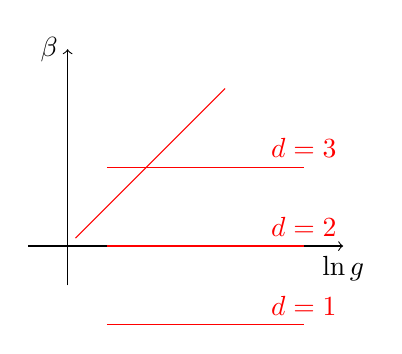
\begin{tikzpicture}
        \draw [->] (-.5,0) -- (3.5,0) node [below] {$\ln g$};
        \draw [->] (0,-.5) -- (0,2.5) node [left] {$\beta$};
        \draw [red] (.1,.1) -- (2,2);
        \draw [red] (.5,1) -- (3,1) node [above] {$d = 3$};
        \draw [red] (.5,0) -- (3,0) node [above] {$d = 2$};
        \draw [red] (.5,-1) -- (3,-1) node [above] {$d = 1$};
      \end{tikzpicture}
    \end{center}
    \begin{enumext}
      \item $d = 1$, for large $g$, $\beta = -1$; for small $g$,
      $\beta = \ln g$. The curve is always negative, and there is no
      the fixed point for $\beta = 0$. The RG always flows to $g \to 0$
      (insulator phase), so all the states are the localized state.
      \item $d = 2$, for large $g$, $\beta = 0$; for small $g$,
      $\beta = \ln g < 0$. The curve is always non-positive, and there is no
      the fixed point for $\beta = 0$. So all the states are the
      localized state.
      \item $d = 3$, for large $g$, $\beta = 1 > 0$; for small $g$,
      $\beta = \ln g < 0$. The curve ranges from positive to negative, so there
      must have an intersection $g_c$ at the $\beta = 0$-axis, this point is the
      fixed point for RG. When $g > g_c$, $\beta > 0$, $g$ increases as $L$
      increases and the system flows to the metal phase;
      when $g < g_c$, the system flows to the insulator phase.
      So, there exists the metal-insulator phase transition when $d = 3$.
    \end{enumext}
  \end{enumext}
\end{solution}